% !TEX TS-program = pdflatex
% !TEX encoding = UTF-8 Unicode

% This is a simple template for a LaTeX document using the "article" class.
% See "book", "report", "letter" for other types of document.

\documentclass[11pt]{article} % use larger type; default would be 10pt

\usepackage[utf8]{inputenc} % set input encoding (not needed with XeLaTeX)

%%% PAGE DIMENSIONS
\usepackage{geometry} % to change the page dimensions
\geometry{a4paper} % or letterpaper (US) or a5paper or....

\usepackage{graphicx} % support the \includegraphics command and options

\usepackage{amssymb}
\usepackage{amsmath}
%%% PACKAGES
\usepackage{booktabs} % for much better looking tables
\usepackage{array} % for better arrays (eg matrices) in maths
\usepackage{paralist} % very flexible & customisable lists (eg. enumerate/itemize, etc.)
\usepackage{verbatim} % adds environment for commenting out blocks of text & for better verbatim
\usepackage{subfig} % make it possible to include more than one captioned figure/table in a single float
% These packages are all incorporated in the memoir class to one degree or another...

%%% HEADERS & FOOTERS
\usepackage{fancyhdr} % This should be set AFTER setting up the page geometry
\pagestyle{fancy} % options: empty , plain , fancy
\renewcommand{\headrulewidth}{0pt} % customise the layout...
\lhead{}\chead{}\rhead{}
\lfoot{}\cfoot{\thepage}\rfoot{}

%%% SECTION TITLE APPEARANCE
\usepackage{sectsty}
\allsectionsfont{\sffamily\mdseries\upshape} % (See the fntguide.pdf for font help)
% (This matches ConTeXt defaults)

%%% ToC (table of contents) APPEARANCE
\usepackage[nottoc,notlof,notlot]{tocbibind} % Put the bibliography in the ToC
\usepackage[titles,subfigure]{tocloft} % Alter the style of the Table of Contents
\renewcommand{\cftsecfont}{\rmfamily\mdseries\upshape}
\renewcommand{\cftsecpagefont}{\rmfamily\mdseries\upshape} % No bold!

\usepackage{amsmath}
\usepackage{graphicx}
\graphicspath{ {./pings/} }
\DeclareMathOperator*{\argmax}{arg\,max}
\DeclareMathOperator*{\argmin}{arg\,min}

\newcount\colveccount
\newcommand*\colvec[1]{
        \global\colveccount#1
        \begin{pmatrix}
        \colvecnext
}
\def\colvecnext#1{
        #1
        \global\advance\colveccount-1
        \ifnum\colveccount>0
                \\
                \expandafter\colvecnext
        \else
                \end{pmatrix}
        \fi
}

%%% END Article customizations

%%% The "real" document content comes below...

\title{Micro HW3}
\author{Michael B. Nattinger\footnote{I worked on this assignment with my study group: Alex von Hafften, Andrew Smith, Ryan Mather, and Tyler Welch. I have also discussed problem(s) with Emily Case, Sarah Bass, Katherine Kwok, and Danny Edgel.}}

%\date{} % Activate to display a given date or no date (if empty),
         % otherwise the current date is printed 

\begin{document}
\maketitle

\section{Question 1}
The TA must be paid $M$ dollars. For a given class size with $n$ students, the total utility is:
\begin{align*}
U = \begin{cases} nm, \text{no TA} \\ na + nm - M, \text{TA} \end{cases}
\end{align*}

It is optimal to pay for the TA if $m\leq a+m-M/n \Rightarrow 0 \leq a-M/n \Rightarrow n\geq M/a.$ Therefore, it is optimal to pay for the TA for $n\geq N$ where $N = M/a.$

\section{Question 2}

The social planner's problem is represented by the following Lagrangian:
\begin{align*}
\mathcal{L} &= x_L^2/2 + x_H^2/2 +(H - b- x_H)x_H + (L - b - x_L)x_L - \beta\bar{x} + \lambda_H(\bar{x} - x_H) + \lambda_L(\bar{x} - x_L)
\end{align*}

Our Kuhn-Tucker conditions are the following:
\begin{align*}
H - x_H - b &= \lambda_H\\
L - x_L - b &= \lambda_L\\
\lambda_H + \lambda_L &= \beta \\
x_H \leq \bar{x},\lambda_H\geq 0, \lambda_H(\bar{x} - x_H) &= 0\\
x_L \leq \bar{x},\lambda_L\geq 0, \lambda_L(\bar{x} - x_L) &= 0
\end{align*}

If $\lambda_L = 0, \lambda_H = \beta = h - x_H - b, x_L = L - b$. Moreover, $\bar{x} = x_H,$ and since $x_L = L-b < \bar{x} = H - b - \beta \rightarrow \beta<H-L. $ Therefore, if $\beta<H-L,$ then our efficient prices are $p^*_H = H - x_H = b+\beta, p^*_{L} = L - x_L = b.$

If $\lambda_L,\lambda_H > 0, x_L = \bar{x} = x_H.$ Then, $\beta =  H - x_H - b + L - x_L - b = H + L -2b - 2\bar{x} \Rightarrow \bar{x} = \frac{H+L - \beta}{2} - b \Rightarrow p_H =  \frac{H-L + \beta}{2} + b, p_L = \frac{L-H+\beta}{2} +b,$ if $\beta\geq H-L$
\section{Question 3}
The Edgeworth box is drawn below, with the endowment labeled with a red star. The contract curve is also drawn in red on the graph, with the result being a line that sets consumer B's consumption in periods 1 and 2 to be equal, due to that agent's utility curve being Leontief. We further plot the results from part (c) in blue.

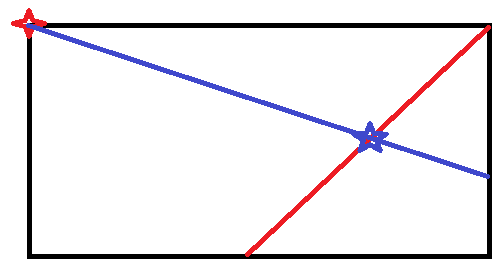
\includegraphics{edgeworth}

We can now solve for the interest rate and endowment.

\begin{align*}
\mathcal{L}^A &= c_1^1c_2^2 - \lambda_A (p_1c_1^1 + p_2c_2^1 - 100p_2),\\
c_1^2 = c_2^2, p_1c_1^2+p_2c_2^2 &= 200p_1,\\
c_1^1 + c_1^2 = 200, c_2^1 + c_2^2 &= 100.
\end{align*} 

Taking FOCs of the Lagrangian,
\begin{align*}
c_2^1 &= \lambda p_1 \\
c_1^1 &= \lambda p_2\\
c_2^1 &= c_1^1 p_1/p_2,\\
c_1^2 &= \frac{200}{1+p_2/p_1}, \\
c_1^1 &= 50 p_2/p_1,\\
50p_2/p_1 + \frac{200}{1+p_2/p_1} &= 200\\
(1/4)(p_2/p_1) + 1/(1+p_2/p_1) &= 1\\
(1/4)(p_2/p_1)^2 + (1/4)(p_2/p_1) +1 - 1 - p_2/p_1 &= 0  \\
(1/4)(p_2/p_1) &= 3/4,\\
p_2/p_1 &= 3.
\end{align*}
Given the interest rate $p_2/p_1 = 3,$
\begin{align*}
c_1^1 &= 150,\\
c_2^1 &= 50, \\
c_1^2 &= 50, \\
c_2^2 &= 50.
\end{align*}

\section{Question 4}
Our optimality for the first consumer is the following:
\begin{align*}
\mathcal{L} &=
\end{align*}
\end{document}
